\documentclass[10.7pt,]{article}

%in the preamble
%--------------------------------
\usepackage[
backend=biber,
style=numeric,
sorting=none,
maxbibnames=3,
]{biblatex}

% supress pp. and add a semi-colon
\DefineBibliographyStrings{english}{%
  page             = {:\ifbibliography{}{}},
  pages            = {:\ifbibliography{}{}},
} 
\renewcommand*{\ppspace}{}

% Supresses In in the bibliographics
\renewbibmacro{in:}{}

\renewbibmacro*{journal+issuetitle}{%
  \usebibmacro{journal}%
  \setunit*{\addspace}%
  \iffieldundef{series}
    {}
    {\newunit
     \printfield{series}%
     \setunit{\addspace}}%
  \setunit{\addspace}%
  \usebibmacro{issue+date}%
  \setunit{\addcolon\space}%
  \usebibmacro{issue}%
  \setunit{\addsemicolon}%
  \usebibmacro{volume+number+eid}%
  \newunit}

\DeclareFieldFormat[article,periodical]{number}{\mkbibparens{#1}}
\renewbibmacro*{volume+number+eid}{%
  \printfield{volume}%
  \printfield{number}%
  \setunit{\addcomma\space}%
  \printfield{eid}}

\renewbibmacro*{issue+date}{%
  \iffieldundef{issue}
    {\usebibmacro{date}}
    {\printfield{issue}%
     \setunit*{}%
     \usebibmacro{date}}%
  \newunit}
  
\renewcommand*{\bibpagespunct}{}
 
\addbibresource{literature.bib}
%--------------------------------
%\usepackage[numbers]{natbib}
%\bibliographystyle{dcu}
%\bibpunct{[}{]}{;}{n}{}{,}


\usepackage[letterpaper, margin=2.54cm, top=2.54cm]{geometry}
\usepackage{lmodern}
\usepackage{authblk} % To add affiliations to authors
\usepackage{amssymb,amsmath}
\usepackage{wrapfig}
\usepackage{graphicx,grffile}
\usepackage[labelfont=bf,labelsep=period]{caption}
\usepackage{ifxetex,ifluatex}
\usepackage{bm}
\usepackage{array, boldline, makecell, booktabs}
\usepackage{multirow}


%\usepackage{fixltx2e} % provides \textsubscript
\ifnum 0\ifxetex 1\fi\ifluatex 1\fi=0 % if pdftex
  \usepackage[T1]{fontenc}
  \usepackage[utf8]{inputenc}
\else % if luatex or xelatex
  \ifxetex
    \usepackage{mathspec}
  \else
    \usepackage{fontspec}
  \fi
  \defaultfontfeatures{Ligatures=TeX,Scale=MatchLowercase}
    \setmainfont[]{Arial Narrow}
    \setsansfont[]{Century Gothic}
    \setmonofont[Mapping=tex-ansi]{Consolas}
\fi
% use upquote if available, for straight quotes in verbatim environments
\IfFileExists{upquote.sty}{\usepackage{upquote}}{}
% use microtype if available
\IfFileExists{microtype.sty}{%
	\usepackage{microtype}
	\UseMicrotypeSet[protrusion]{basicmath} % disable protrusion for tt fonts
}{}



%==============================
% Customization to make the output PDF 
% look similar to the MS Word version
%==============================
% To prevent hyphenation
\hyphenpenalty=10000
\exhyphenpenalty=10000

% To set the sections font size
\usepackage{sectsty}
\allsectionsfont{\fontsize{11}{11}\selectfont}
\sectionfont{\fontsize{14}{14}\selectfont}
\subsectionfont{\bfseries\fontsize{13}{13}\selectfont}
\subsubsectionfont{\bfseries\fontsize{11}{11}\selectfont}
%\subsubsectionfont{\normalfont}

% Spacing
\usepackage{setspace}

\usepackage{xcolor}

\usepackage{dsfont}
\usepackage{amsmath,amssymb}
\DeclareMathOperator*{\argmax}{arg\,max}
\DeclareMathOperator*{\argmin}{arg\,min}


% No new line after subsubsection
\makeatletter
%\renewcommand\subsubsection{\@startsection{subsubsection}{3}{\z@}%
%	{-3.25ex\@plus -1ex \@minus -.2ex}%
%    {-1.5ex \@plus -.2ex}% Formerly 1.5ex \@plus .2ex
%    {\normalfont}}
%\makeatother

% To set the doc title font
\usepackage{etoolbox}
\makeatletter
\patchcmd{\@maketitle}{\LARGE}{\bfseries\fontsize{15}{16}\selectfont}{}{}
\makeatother

% No page numbering
\pagenumbering{gobble}

\makeatletter
\def\maxwidth{\ifdim\Gin@nat@width>\linewidth\linewidth\else\Gin@nat@width\fi}
\def\maxheight{\ifdim\Gin@nat@height>\textheight\textheight\else\Gin@nat@height\fi}
\makeatother

% Scale images if necessary, so that they will not overflow the page
% margins by default, and it is still possible to overwrite the defaults
% using explicit options in \includegraphics[width, height, ...]{}
\setkeys{Gin}{width=\maxwidth,height=\maxheight,keepaspectratio}
\setlength{\parindent}{0pt}
\setlength{\parskip}{6pt plus 2pt minus 1pt}
\setlength{\emergencystretch}{3em}  % prevent overfull lines
\providecommand{\tightlist}{%
  \setlength{\itemsep}{0pt}\setlength{\parskip}{0pt}}
\setcounter{secnumdepth}{0}
% Redefines (sub)paragraphs to behave more like sections
\ifx\paragraph\undefined\else
\let\oldparagraph\paragraph
\renewcommand{\paragraph}[1]{\oldparagraph{#1}\mbox{}}
\fi
\ifx\subparagraph\undefined\else
\let\oldsubparagraph\subparagraph
\renewcommand{\subparagraph}[1]{\oldsubparagraph{#1}\mbox{}}
\fi
%==============================
\usepackage{hyperref}
\hypersetup{
	unicode=true,
	pdftitle={My Cool Title Here},
	pdfauthor={Author One, Author Two, Author Three},
	pdfkeywords={keyword1, keyword2},
	pdfborder={0 0 0},
	breaklinks=true
}
\urlstyle{same}  % don't use monospace font for urls

% Keywords command
\providecommand{\keywords}[1]
{
  \small	
  \textbf{Key words---} #1
}
%==============================

% reduce space between title and beginning of page
\title{Not So Weak-PICO: Leveraging weak supervision for Participants, Interventions, and Outcomes recognition for systematic review automation}
\date{} % \vspace{-2em}
\author[ ] {
    % Authors
    \bf\fontsize{13}{14}\selectfont
    Anjani Dhrangadhariya\textsuperscript{\rm 1, 2},
    Henning M\"uller \textsuperscript{\rm 1, 2}
}
\affil[1]{Informatics Institute, University of Applied Sciences Western Switzerland (HES-SO), Sierre, Switzerland}
\affil[2]{University of Geneva (UNIGE), Geneva, Switzerland}
\affil[*]{Corresponding author: Anjani Dhrangadhariya, Rue de Technopôle 3, Informatics Institute, University of Applied Sciences Western Switzerland (HES-SO), 3960 Sierre, Switzerland; anjani.dhrangadhariya@hevs.ch; +41 58 606 90 03}
%==============================
\begin{document}
\maketitle
%\vspace{2em} %separation between the affiliations and abstract
%==============================
\doublespacing
%==============================

Word count: 3798 %Anjani TODO - Update before submission

\clearpage
\section{\textbf{ABSTRACT}}
\label{abstract}
%==============================
% Note: Abstract is limited to 250 words
%
\textbf{Objective:}
PICO (Participants, Interventions, Comparators, Outcomes) analysis is vital but time-consuming for conducting systematic reviews (SRs). 
Supervised machine learning can help fully automate it, but a lack of large annotated corpora limits the quality of automated PICO recognition systems.
The largest currently available PICO corpus is manually annotated, which is an approach that is often too expensive for the scientific community to apply.
Depending on the specific SR question, PICO criteria are extended to PICOS (S-Study type or design), PICOC (C-Context), and PICOT (T-timeframe), meaning the static hand-labelled corpora need to undergo costly re-annotation as per the downstream requirements.
We aim to test the feasibility of designing a weak supervision system to extract these entities without hand-labelled data.
\textbf{Methodology:}
We use multiple medical and non-medical ontologies and expert-generated rules to obtain labels for PICO entities.
These labels were aggregated using simple majority voting and generative modelling.
The resulting programmatic labels were used as weak signals to train a weakly-supervised discriminative model and observe performance changes.
Additionally, we explore mistakes in the currently available PICO test set that could have led to inaccurate evaluation of several automation methods.
\textbf{Results:}
We present Weak-PICO, a weakly-supervised PICO entity recognition approach using medical ontologies, non-medical ontologies and various expert-generated rules and dictionaries.
Unlike manual annotation, Weak-PICO does not use hand-labelled data and is quickly adaptable and extensible to other entities.
\textbf{Conclusion:}
Weak supervision using weak-PICO for PICO entity recognition has encouraging results and readily extends to more clinical entities.


\keywords{Weak supervision, Machine learning, Information extraction, Evidence-based Medicine}
%
\clearpage
% Full paper is limited to 4000 words (approx. 14.6 pages)
%
%==============================
\section{\textbf{INTRODUCTION}}\label{introduction}
%==============================
%
Systematic Reviews (SR) are an evidence-based practice of answering clinical questions using a transparent and quantitative approach.
The reviewers must collect as many candidate publications as possible, identifying the relevant ones from these and integrating their results via statistical meta-analysis.
Filtering relevant publications from non-relevant publications with similar keywords often uses PICO (Participants, Interventions, Comparators, Outcomes) criteria. 
A clinical study or a publication is only relevant for answering a question if it studies the selected participants, interventions (and their comparators) and outcomes.~\cite{uman2011systematic} 
Manually analyzing PICO information from thousands of publications for a single SR often takes about 12 months of two medical experts' time.
The process can be automated using machine learning (ML) by directly pointing the human reviewers to the correct text chunks describing PICO.
Hand labelling corpora with PICO information requires people with combined medical and informatics skills, which is expensive and time-consuming in terms of the actual annotation process and annotator training.

Labelling PICO information is tricky because of the high disagreement between human annotators on the exact spans constituting PICO, leading to human errors in hand-labelled corpora.~\cite{brockmeier2019improving}
Additionally, depending upon the systematic review question, PICO criteria are extended to PICOS (S-Study design), PICOC (C-Context), and PICOT (T-timeframe).~\cite{riva2012your,methley2014pico,uman2011systematic}
Hand-labelled datasets are static and prohibit quick manual re-labelling in case of human errors or when a downstream task requires new entities.
In SRs, the step after PICO information analysis is to identify the risk of bias from the studies, which is another information extraction lacking a manually labelled corpus. 
This annotation bottleneck has pivoted attention towards weakly-supervised learning that relies on programmatic labelling sources to obtain training data.
Programmatic labelling is quick and allows efficient modifications to the training data labels per the downstream application changes.

Weakly-supervised (WS) learning has demonstrated strengths for clinical document classification and relation extraction, but clinical entity extraction tasks have heavily relied on fully-supervised (FS) approaches.~\cite{meng2018weakly,wang2019clinical,mintz2009distant,elangovan2020assigning,weber2020pedl,mallory2020extracting}
Despite the availability of UMLS, a large compendium of medical ontologies, which can be re-purposed for weak entity labelling, it has not been extensively applied to clinical entity labelling.~\cite{humphreys1998unified}
Several legacy clinical applications are also supported by rule-based \textit{if-else} systems relying on keyword cues that aid weak labelling.~\cite{friedlin2008software,kim2017extracting,yang2015automatic}
With so many weak labelling sources available, the challenge for weak supervision is efficiently aggregating these sources of varying accuracy.


Data programming is a domain agnostic generative modelling approach combining multiple weak labelling sources and estimating their accuracies.
The effectiveness of data programming for biomedical entity recognition has been explored by Fries \textit{et al.} in their Trove system.
However, Trove only explores the well defined entities like chemical, disease, disorder and drug classes.~\cite{fries2021ontology}
PICO categories are text spans by definition, fuzzier in comparison and much more intricate in that they can be divided into subclasses.
A shortcoming of span extraction is that even after a machine points a human reviewer to the correct PICO span, the reviewer requires to manually read and understand its finer aspects to screen the study for relevance.
Span extraction hence leads to semi-automation but hinders full-automation.
The entity recognition approach to PICO is not as easy as the entity recognition approach to disease or chemical names which are more or less standardized.
These terms are not standard, and even the experts disagree on the exact tokens constituting PICO.~\cite{brockmeier2019improving}
Weakly-supervised PICO entity recognition has not garnered as much attention as supervised span recognition.
As far as our knowledge goes, only two studies exist for weakly-supervised PICO recognition.
One of these approaches only explores distant supervision for intervention extraction using a single labelling source, and the other relies on a single source of programmatic labelling and focuses on PICO spans and sentences rather than entities.~\cite{liu2021sent2span,dhrangadhariya2022distant}

The challenges to developing weak supervision approaches to PICO entity recognition are first defining the subclasses within PICO spans and then mapping several available ontologies and terminologies to these.
The next challenge is developing weakly-supervised classifiers by optimally combining several ontologies and evaluating their performance compared to full supervision.
Another challenge is developing higher-cost expert-generated rules corresponding to these subclasses to aid ontology classifiers and evaluate their combined performance.
We also identified limitations in the currently available EBM-PICO training dataset and corrected them for reliable evaluation of the WS approaches.
This work demonstrates the feasibility of using weak supervision for PICO entity extraction using the EBM-PICO benchmark.
We show how using only ontology-dependent classifiers vs. combining them with more expensive expert-generated rules compares to fully-supervised extraction and, in some instances overtaking it.
%
%==============================
\section{\textbf{METHODOLOGY}}\label{methods}
%==============================
%
The birds-eye view of our approach is shown in the Figure~\ref{fig:approach}.
%
\begin{figure}[ht]
\centering
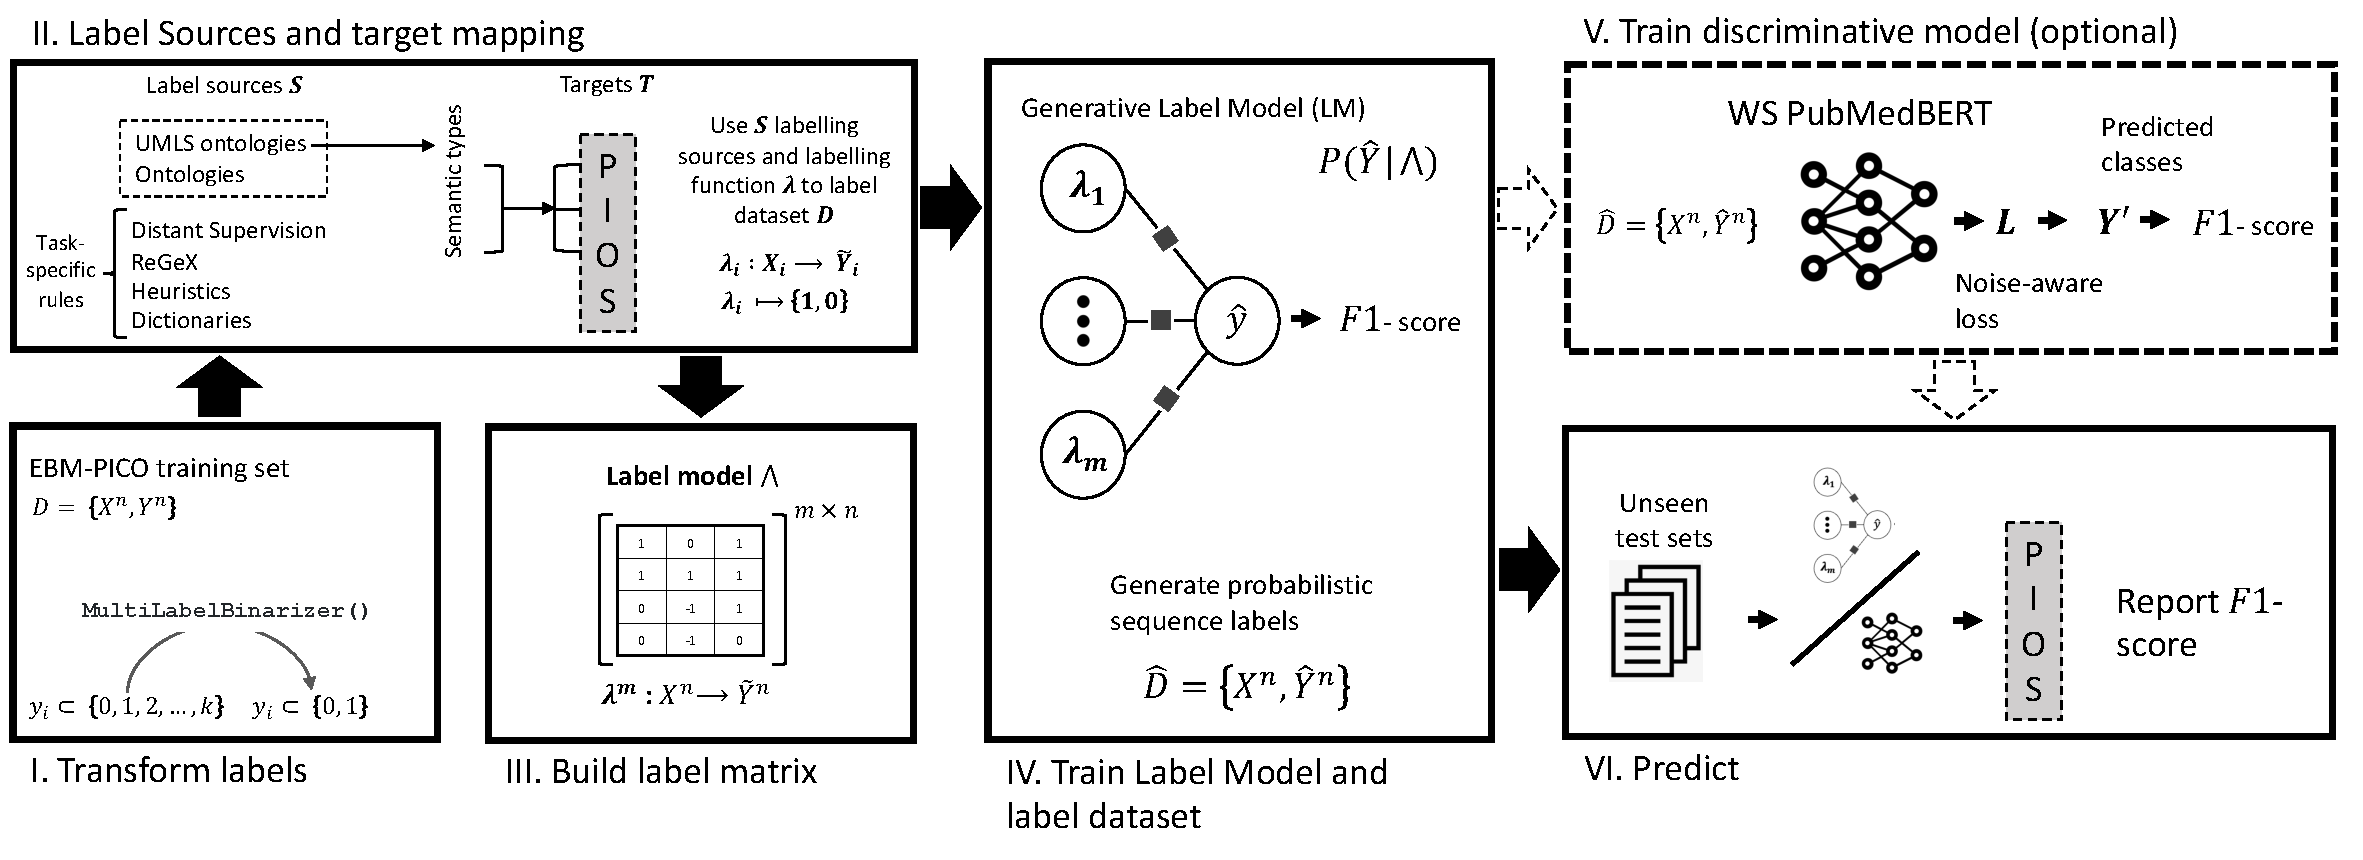
\includegraphics[width=0.98\textwidth]{figures/approach.pdf}
\caption{Weak PICO entity extraction approach: I) Multi-class labels in the EBM-PICO benchmark are binarized. II) Low-cost UMLS vocabularies are repurposed as labelling sources and experts design rules as high-cost labelling courses. III) Labelling functions map the training sequences to class labels using labelling sources resulting in an $m \times n$ label matrix. IV-V) The label matrix is used to train a generative model that outputs probabilistic labels that a downstream transformer model can use for entity recognition.}
\label{fig:approach}
\end{figure}
%
%==============================
\subsection{datasets}\label{data}
%==============================
%
EBM-PICO is a widely used dataset with PICO annotations at two levels: span-level or coarse-grained and entity-level or fine-grained (see Table~\ref{tab:coarsefineconcept}).
Span-level annotations encompass the maximum information about each class.
Entity-level annotations cover the more fine-grained information at the entity level, with PICO classes further divided into fine-grained subclasses.
The dataset comes pre-divided into a training set (n=4,933) annotated through crowd-sourcing and an expert annotated gold test set (n=191) for evaluation.~\cite{nye2018corpus}

The EBM-PICO annotation guidelines caution about variable annotation quality~\footnote{\url{https://www.ncbi.nlm.nih.gov/pmc/articles/PMC6174533/bin/NIHMS988059-supplement-Appendix.pdf}}.
Low annotation quality in the training dataset is excusable, but the errors in the test set can lead to faulty evaluation of the downstream ML methods.
We evaluate 1\% of the EBM-PICO training set tokens to gauge the possible reasons for the fine-grained labelling errors and use this exercise to conduct an error-focused PICO re-annotation for the EBM-PICO gold test set.
The dataset is pre-tokenized and did not require additional preprocessing except the addition of POS tags and token lemma using spaCy~\footnote{\url{https://spacy.io/}}.
Multi-class fine-grained PICO annotations were binarized, i.e. a token label was reset to 1 if the token represented a fine-grained entity.
%
\begin{table}[h!]
\begin{center}
\begin{tabular}{| c | c | c | c |} 
\hline
 & P & I/C & O \\ 
\hline
0 & No label & No label & No label \\ 
1 & Age & Surgical & Physical \\ 
2 & Sex & Physical & Pain \\
3 & Sample size & Drug & Mortality \\
4 & Condition & Educational & Side effect \\
5 &  & Psychological & Mental \\
6 &  & Other & Other \\
7 &  & Control &  \\
\hline
\end{tabular}
\caption{\label{tab:coarsefineconcept} P (Participant), I (Intervention) and O (Outcome) represent the coarse-grained labels that are further divided into respective fine-grained labels. The table is taken from Nye \textit{et al.}~\cite{nye2018corpus}}
\end{center}
\end{table}
%
%==============================
\subsection{sequence labeling}\label{seq_lab}
%==============================
%
Automatic PICO entity labelling is a classical binary sequence labelling problem whereby a function maps an input sequence of n text tokens, $ \bm{X} = (x_{1}, x_{2}, \dotso , x_{n} )$ to output sequence $\bm{Y} = (y_{1}, y_{2}, \dotso , y_{n} )$, where $y_{i} \subset y; y = \{1,0\} $ is the label for token $x_{i}$.
In weak supervision, $\bm{Y}$ is latent and should be estimated by aggregating several weak labelers of variable accuracy.
The estimates $\bm{\hat{Y}}$ of $\bm{Y}$ are assigned as probabilistic token labels of $\bm{X}$ leading to a weakly labelled dataset that can be used to train discriminative models.
%
%==============================
\subsection{labelling sources}\label{lss}
%==============================
%
We used the 2021AB-full release of the UMLS Metathesaurus English subset with 223 vocabularies.
After removing non-English and zoonotic vocabularies and the vocabularies containing fewer than 500 terms, we remained with 127 vocabularies.~\cite{humphreys1998unified}
Terms in the selected vocabularies were preprocessed by removing stopwords, numbers, and punctuation.
Additional vocabularies included disease ontology (DO), Human Phenotype Ontology (HPO), Ontology of adverse events (OAE), Chemical entities of biological interest (ChEBI),  comparative toxicogenomics database (CTD) Chemical and Disease subclasses, Clinical Trials Ontology (NDD-CTO), Gender, Sex, and Sexual Orientation Ontology (GSSO), Chemotherapy Toxicities Ontology (ONTOTOX), Cancer Care: Treatment Outcomes Ontology (CCTOO), symptoms ontology (SYMP), Non-pharmacological interventions ontology (NPI), Nursing Care Coordination Ontology (NCCO).~\cite{schriml2012disease,robinson2008human,he2014oae,de2010chemical,lin2020cto,kronk2020development,geifman2011towards,rogier2021using,lin2018cancer,mohammed2012building,ninot2018definition}
Regular expressions (ReGeX) and heuristics like POS tag cues were used to capture recurring class-specific patterns otherwise not captured by standardized terminologies.
The hand-coded dictionaries were designed using the official websites listing patient-reported outcome (PROMs) questionnaires~\footnote{\url{https://www.thoracic.org/members/assemblies/assemblies/bshsr/patient-outcome/}} and PROMs~\footnote{\url{https://www.safetyandquality.gov.au/our-work/indicators-measurement-and-reporting/patient-reported-outcomes/proms-lists}}.
Vocabularies are structured, standardized data sources that do not capture writing variations from clinical literature and custom-built ReGeX are restricted by either task or entity type.~\cite{ratner2017snorkel,safranchik2020weakly}
We used distant supervision dictionaries created from the structured fields of clinicaltrials.gov (CTO) as described by Dhrangadhariya \textit{et al.}~\cite{dhrangadhariya2022distant}
Principal investigators of the clinical study manually enter data in CTO, thereby incorporating large-scale writing variations.  
%
%
%
%==============================
\subsection{Labeling functions}\label{lfs}
%==============================
%
In a binary token labelling task, a labelling function is a weak classifier $\lambda$ that uses domain-specific labelling sources $\bm{S}$ and a logic to emit token labels $ \widetilde{\bm{Y_{i}}}$ with labels $ \widetilde{y} \in \{-1, 0, +1\}$ for a subset of input $\bm{X_{i}}$ tokens.
A labelling function designed for a particular target class $t \in \bm{T}$ (here; $\bm{T} \subset \{ Participant, Intervention, Outcome \} $) should output  $1$ for the positive token label, $0$ for the negative token label, and abstain ($-1$) on the tokens where it is uncertain $\lambda \mapsto \{-1, 0, +1\}$.
We designed three LF types depending on the types of labelling sources.
The ontology or dictionary labelling functions for a target class take a dictionary of terminologies mapped to one of $y \subset \{0, +1\} $ token labels.
Any labelling function using ontologies or dictionaries used string matching as the labelling heuristic.
Relevant bigram word co-occurrences were used to account for fuzzy span matching from the terminologies.
A ReGeX labelling function for a target class takes regex patterns for $\{-1, +1\}$ labels and abstains from the rest.
A heuristic labelling function is personalized for each target class and takes a generic regex pattern and specific POS (part-of-speech) tag signals.
Abbreviations in clinical studies are considered using a heuristics abbreviation identifier, and the identified abbreviations were mapped to their respective target classes.
Stopwords from Natural Language Tookit (NLTK)~\footnote{\url{https://www.nltk.org}}, spaCy, Gensim~\footnote{\url{https://radimrehurek.com/gensim/}}, and scikit learn~\footnote{\url{https://scikit-learn.org}} were used to initialize negative token label templates.
%
%
%
%==============================
\subsection{sources to targets}\label{s2t}
%==============================
%
UMLS concepts are organized under semantic type categories (e.g. disease, sign and symptoms, age group, etc.)~\footnote{\url{https://www.nlm.nih.gov/research/umls/META3_current_semantic_types.html}}, so mapping these semantic categories to PICO targets invariably maps the concepts from the vocabularies to target classes.
It is a challenging expert-led activity, though decomposing PICO into subclasses greatly helps map sources to target.
A semantic category was either marked $\{1, 0\}$ depending upon its relevance to the target class (refer to Supplementary material section on UMLS sources to PICO targets).
Non-UMLS vocabularies were obtained from NCBO bioportal~\footnote{\url{https://bioportal.bioontology.org/}} and were chosen to be PICO target specific and assigned to a single label.
Target-specific distant supervision dictionaries were created from the structured fields of clinicaltrials.gov (CTO). 
The structured field ``Condition or Disease'' was mapped to the Participant target, and the ``Intervention/Treatment'' field was mapped to the Intervention target.
The semi-structured ``Primary Outcome Measures'' and ``Secondary Outcome Measures'' fields were mapped to the Outcomes class.
Hand-crafted dictionaries were separately designed for participant gender, intervention comparator terms and outcomes.
%
%
%
%==============================
\subsection{LF aggregation}\label{lms}
%==============================
%
Each labelling function $ \lambda_{i} \in \bm{\Lambda^{m}}; \bm{\Lambda} = \{\lambda_{1}, \lambda_{2}, \dotso, \lambda_{m} \} $ maps a subset of inputs $\bm{X^{n}}$ to output sequence $ \widetilde{\bm{Y^{n}}}$ with labels $\widetilde{y} \in \{-1, 0, +1\}$ yielding a label matrix $ \lambda \subset \{-1, 0, +1\}^{m \times n}$.
The weakly-generated labels might have conflicts and overlaps and are generally noisy in nature.
The labelling functions can be ensembled using the majority vote (MV) rule, where a token label is elected only when a majority of $\lambda_{i}$ vote for it.
Ties and abstains lead to the selection of the majority label.
%
\begin{equation}
\bm{\hat{Y_{MV}}} = \max_{{y \subset \{ 0, 1 \} }} \sum_{i=1}^{m} \mathds{1} (\lambda_{i} = y_{i})
\end{equation}
%
However, MV considers each labeling function as conditionally independent and does not take into account the variable accuracies of different labelling sources weighing them equally.
Snorkel implements data programming paradigm into label model (LM) that re-weights and aggregates labelling functions into probabilistic labels $\hat{y_{i}}$.
To do this, label model trains a generative model $ \bm{P} ( \Lambda , Y )$ to estimate LF accuracies $\theta_{j}$ using stochastic gradient descent to minimize log loss in absence of labelled data.~\cite{ratner2017snorkel,dunnmon2020cross}
Even though the ground truth is not observable to estimate accuracies, they can be estimated using observed agreements and disagreements rates between labelling function pairs $ \lambda_{i}, \lambda_{j}$ in $\Lambda$.
Generative modeling ultimately results into token label probablities $\bm{\hat{Y}}$ for label classes $ \{ 0, 1\} $.
GridSearch was used to fine tune the parameters of the label model using the hand-labelled validation set from the EBM-PICO.
The parameters are listed in the Experimental details section of the supplementary material.
Once we have the pseudo-labels generated by majority voting or the label model, these could be used to train a discriminative model.
%
\begin{equation}
\bm{\hat{\theta}} = \argmin_{\theta} \big( -\log \sum_{Y} p_{\theta} (\Lambda , Y ) \big)
\end{equation}
%
%
%
%==============================
\subsection{experiments}\label{subsec:experiments}
%==============================
%
Ontologies are readily-available sources of weak supervision and do not require expert knowledge, while rules require expert investment for development.
We tested whether adding expert-engineered rule-based labelling sources brought performance gains to ontology-based labelling sources.
We report results on three tiers to gauge the performance changes: 1) UMLS labelling sources, 2) UMLS and non-UMLS labelling sources, 3) UMLS, non-UMLS and exert generated rules. 
UMLS ontologies were ranked based on the total number of n-gram overlaps between the respective terminology and EBM-PICO validation set.
The ontologies were partitioned into $s = ( 1, 2, \dotso , 127 )$ partitions with partition one aggregating all the ontologies into a single LF and partition 127 with all the ontologies as separate LFs.



The labelling functions $\lambda_{m}$ were used to label the EBM-PICO training set and obtain $\lambda$. 
We tested MV and LM to aggregate labelling functions.
LM output probabilistic labels for the training set were used as weak supervision signals to train downstream PubMedBERT that was trained to minimize noise-aware cross-entropy loss.
%
\begin{equation}
\bm{\hat{\omega}} = \argmin_{\omega} \frac{1}{N} \sum_{i=1}^{n} \mathbb{ E }_{ \hat{y} \sim \hat{Y}} \big[ l \big( f(x, w), \hat{y} \big) \big]
\end{equation}
%
PubMedBERT was chosen because of its domain similarity to our training data (PubMed abstracts) and task.
It was tuned on fixed parameters listed in the experimental details section in the supplementary material. 
%
%
%
%==============================
\subsection{evaluation}\label{eval}
%==============================
%
We report the classical macro-averaged F1 and recall for MV, LM, weakly-supervised (WS) transformer models and the fully-supervised (FS) transformer models.
Mean macro-averaged scores are reported over three runs of each of these models with the top three random seeds (0, 1, and 42) used in Python.
The models were separately trained for each target class recognition tasks using the raw (IO) tagging scheme.
We used students t-test with a alpha $\alpha$ threshold of 0.05 to measure the statistical significance.
%
%==============================
\section{RESULTS}\label{results}
%==============================
%
Coarse-grained PICO annotations in EBM-PICO are spans composed of multiple fine-grained subclasses (refer to Table~\ref{tab:coarsefineconcept}).
We extended these subclasses to better query the labelling sources and design labelling functions (see Figure~\ref{fig:target_subgroups}).
For a more comprehensive subgrouping, we propose developing a PICO ontology.~\cite{sanchez2022annotated}
It is more straightforward to search for ontologies representing adverse events or diseases rather than fending for an ontology describing the entire participant or outcome spans.
Similarly, it is easier to grasp cues separately for outcome terms and instruments of outcome measurement to develop heuristics.
The intervention span can include intervention name, role (primary intervention or comparator), dosage, frequency, mode of administration and administrator.
The outcome span can include the outcome names, the scales, techniques or instruments used to measure them and the absolute outcome measurement values.
The EBM-NLP guidelines restrict annotating the outcome name and how it was measured and to the intervention's name and role (control, placebo), leaving out the other subclasses.
We designed $m$ labelling functions $\lambda^{m}$ corresponding to these guidelines, aggregated them to get probabilistic token labels, and used the weakly-labelled dataset for downstream PICO recognition tasks.
%
\begin{figure}[ht]
\centering
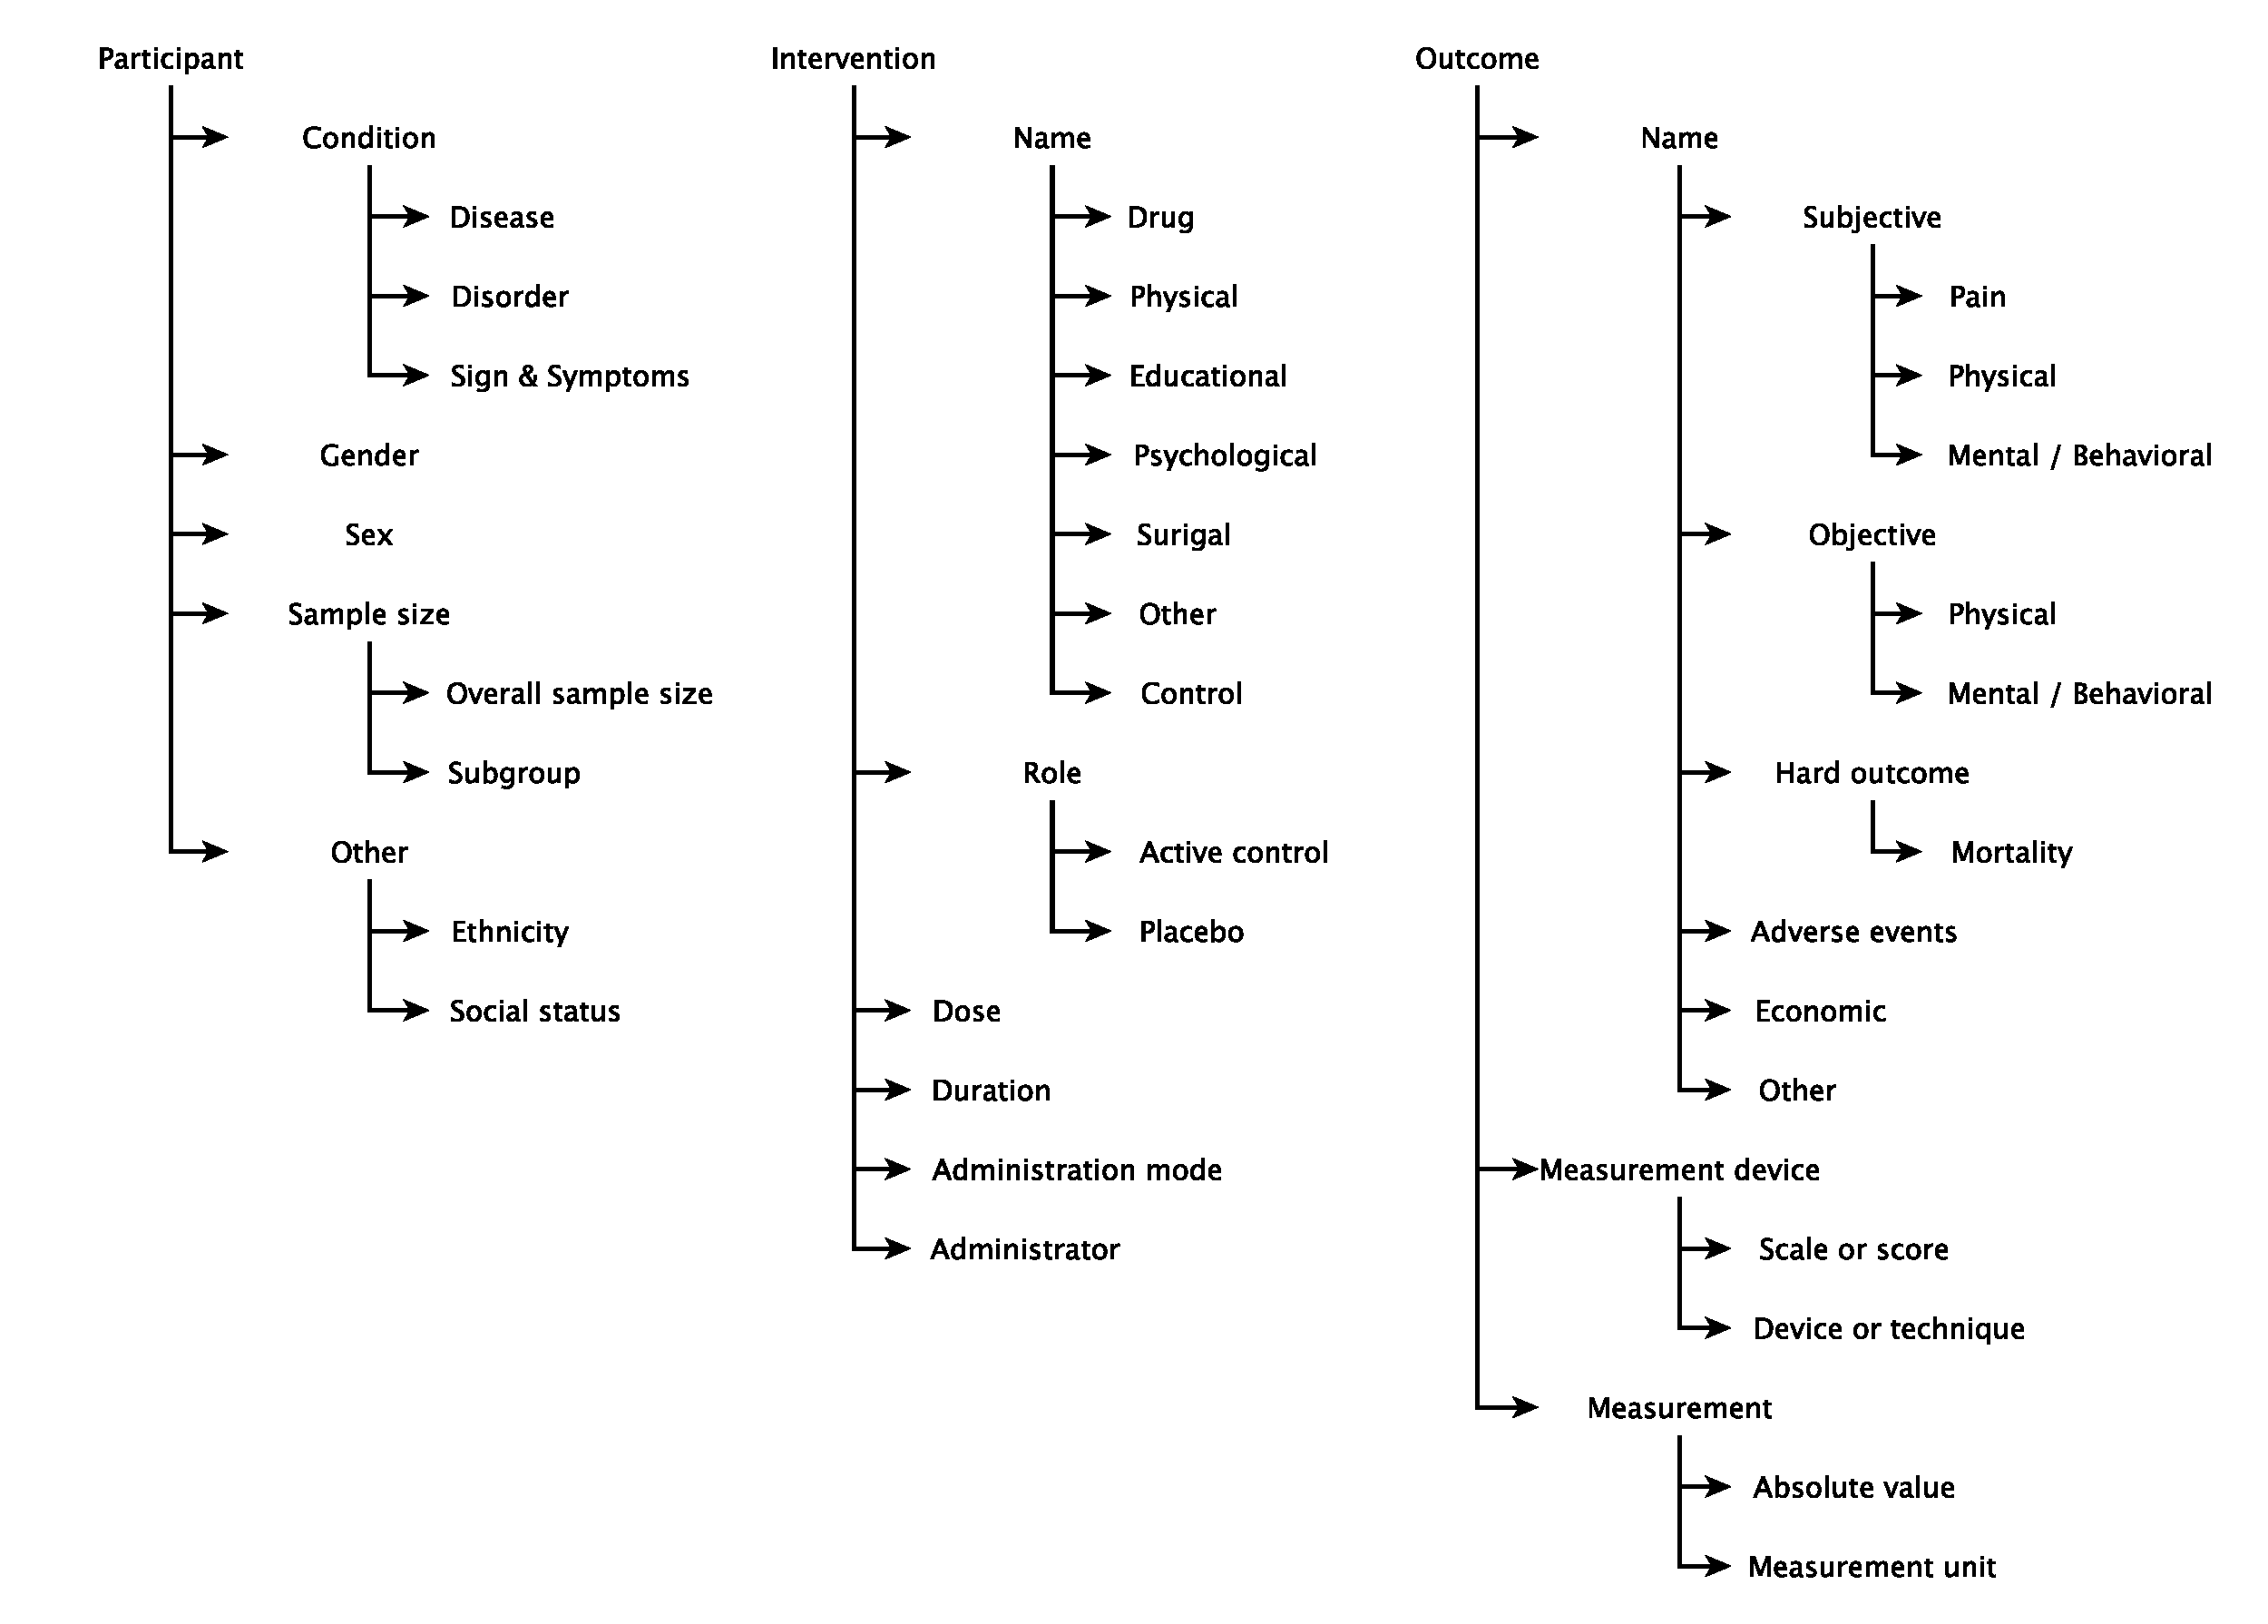
\includegraphics[width=0.95\textwidth]{figures/target_subgroups_.pdf}
\caption{\label{fig:target_subgroups} Hierarchical representation of PICO subclasses. The categories marked in \textbf{\textit{bold-italic}} are the same as the fine-grained categories in EBM-PICO corpus.}
\end{figure}
%
We rectified the errors in EBM-PICO validation set and categorized them for each of the PIO classes as shown in the Table~\ref{tab:errordist}.
Of 12,960 (1\%) training tokens evaluated to gauge the errors, 18.30\% of the Intervention class tokens, 23.39\% of the Participant class tokens and 20.21\% of the Outcome class tokens were errors.
The error analysis was used to correct fine-grained annotation errors in the EBM-PICO test set and both the EBM-PICO and its updated version were used for evaluation.
Table~\ref{tab:res} reports macro-averaged F1 for the experiments detailed in the experiments section in comparison to the fully-supervised approach.
%
\begin{table}[!ht]
    \centering
    \begin{tabular}{|l|r|r|r|}
    \hline
        Error category & Participant & Intervention & Outcome \\ \hline
        Repeat mention unmarked & 213 & 227 & 207 \\ 
        Remain un-annotated & 47 & 59 & 71 \\ 
        Inconsistency & 46 & 18 & 85 \\ 
        Punctuation/article & 15 & 23 & 48 \\ 
        Conjunction connector & 30 & 36 & 57 \\ 
        Junk & 53 & 79 & 30 \\ 
        Extra information & 80 & 146 & 58 \\ 
        Generic mention & 70 & 120 & 85 \\ \hline
        Total errors & 554 & 708 & 641 \\ \hline
    \end{tabular}
    \caption{\label{tab:errordist} Error distribution and error categories in the analysed tokens (1\%) of EBM-PICO corpus.}
\end{table}
%
\begin{table}[!ht]
    \centering
    \begin{tabular}{|l|l|l|l|l|l|l|l|l|l|l|}
        \hline
        \multicolumn{3}{|c|}{} &
        \multicolumn{2}{|c|}{MV} & \multicolumn{2}{|c|}{LM} & \multicolumn{2}{|c|}{WS} & \multicolumn{2}{|c|}{FS} \\
        \hline
        Target & LF source & \#LF & Fine & Corr & Fine & Corr & Fine & Corr & Fine & Corr \\  \hline
        P & UMLS &  & 62.13 & 69.28 & 64.28 & 72.22 & 65.32 & 73.49 & 72.99 & 74.41 \\
         & +Ontology &  & 61.72 & 69.32 & 64.23 & 72.18 & 64.76 & 72.31 &  &  \\ 
         & +Rules &  & 63.08 & 72.06 & 65.79 & 75.31 & 66.73 & \underbar{\textbf{76.12}} &  &  \\ \hline
        I/C & UMLS &  & 59.7 & 63.94 & 60.11 & 64.28 & 59.17 & 61.72 & \textbf{83.37} & 81.06 \\ 
         & +Ontology &  & 62.14 & 66.92 & 62.83 & 67.09 & 67.06 & 69.76 & &  \\
         & +Rules &  & 58.51 & 63.45 & 64.34 & 68.17 & 70.27 & \underbar{72.39} &  &  \\ \hline
        O & UMLS &  & 55.79 & 59.85 & 58.76 & 62.36 & 60.83 & \underbar{63.55} & \textbf{81.2} & 80.53 \\
         & +Ontology &  & 56.006 & 59.64 & 59.27 & 62.34 & 59.55 & 60.46 &  &  \\ 
         & +Rules &  & 55.08 & 59.36 & 60.9 & 62.87 & 60.5 & 60.39 &  &  \\ \hline
    \end{tabular}
    \caption{ Macro-averaged F1 scores for UMLS, UMLS+other and rule-based weak supervision. Underlined values show the best score without manually labelled training data. Note: Fine = EBM-PICO fine-grained annotations, Corr = EBM-PICO fine-grained annotations (updated)}
    \label{tab:res}
\end{table}
%
\paragraph{\textit{error rectification}}
Error rectification leads to an overall average F1 improvement of 4.88\% across the experiments using a weakly labelled training set with the highest average improvement of 8.25\% (7.15\%-9.52\%) for Participants and 2.68\% (-0.11\%-4.28\%) for Outcomes. 
For the Participant class, both the LM and the WS F1 scores increase the full supervision score by 0.90\% - 1.71\%.
It has to be noticed that weak supervision outperforms full supervision on the rectified benchmark only for the participant entity.

\paragraph{\textit{MV vs. LM vs. WS}}
The label model improved the average performance by 2.74\% (0.17\%-5.83\%) in comparison to majority voting.
However, PubMedBERT did not guarantee improved performance across the targets leading to performance drops between 0.4 - 2.56\%.
Though the weakly-supervised PubMedBERT models did not always improve the performance compared to their label model counterparts, they had the best F1 score for each target class.
Majority voting had higher recall across experiments in comparison to precision while LM focused on precision (see Figure~\ref{fig:precRecall}).
%
\begin{figure}
    \centering
    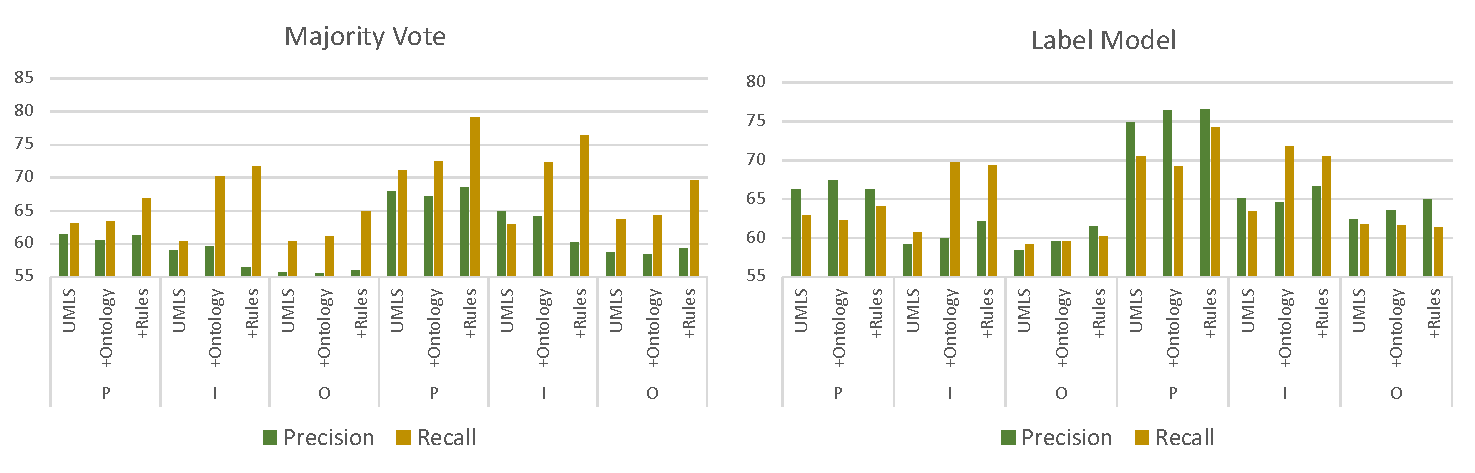
\includegraphics{figures/precRecall.pdf}
    \caption{Precision and recall across the experiments for the I. Majority vote models and II. Label models}
    \label{fig:precRecall}
\end{figure}

\paragraph{\textit{LF tiers}}
Adding non-UMLS LFs to the UMLS tier increases performance for the intervention target by an average of 4.48\%, but leads to performance drops for the participants and outcomes targets by 0.36\% and 0.64\% respectively.
Adding task-specific LF's increased the overall F1 by a negligible 0.98\%.
Heuristics improved performance for interventions LM by 11.1\%.
%
\paragraph{\textit{UMLS partitions}}
To investigate the optimal number of UMLS labelling functions required, we used the same methodology as in Trove holding all non-UMLS and heuristics LFs fixed across all ablation tiers and computed performance across partitions = $s = ( 1, 2, \dotso , 127 )$ partitions of the UMLS by terminology.
We did notice an increasing performance for the first few partitions but did not see the performance drop with a further increase in the partition number for the Participant target.
For the outcomes target, increase in the number of partitions leads to an increased performance initially but drop with further increase in the partition numbers.
This is in contrast to Trove where increase in partitions leads to a drop in performance across targets (refer Figure~\ref{fig:partitions}).
Notice that LM outperforms MV on training performance across the targets and experiments.
%
\begin{figure}
    \centering
    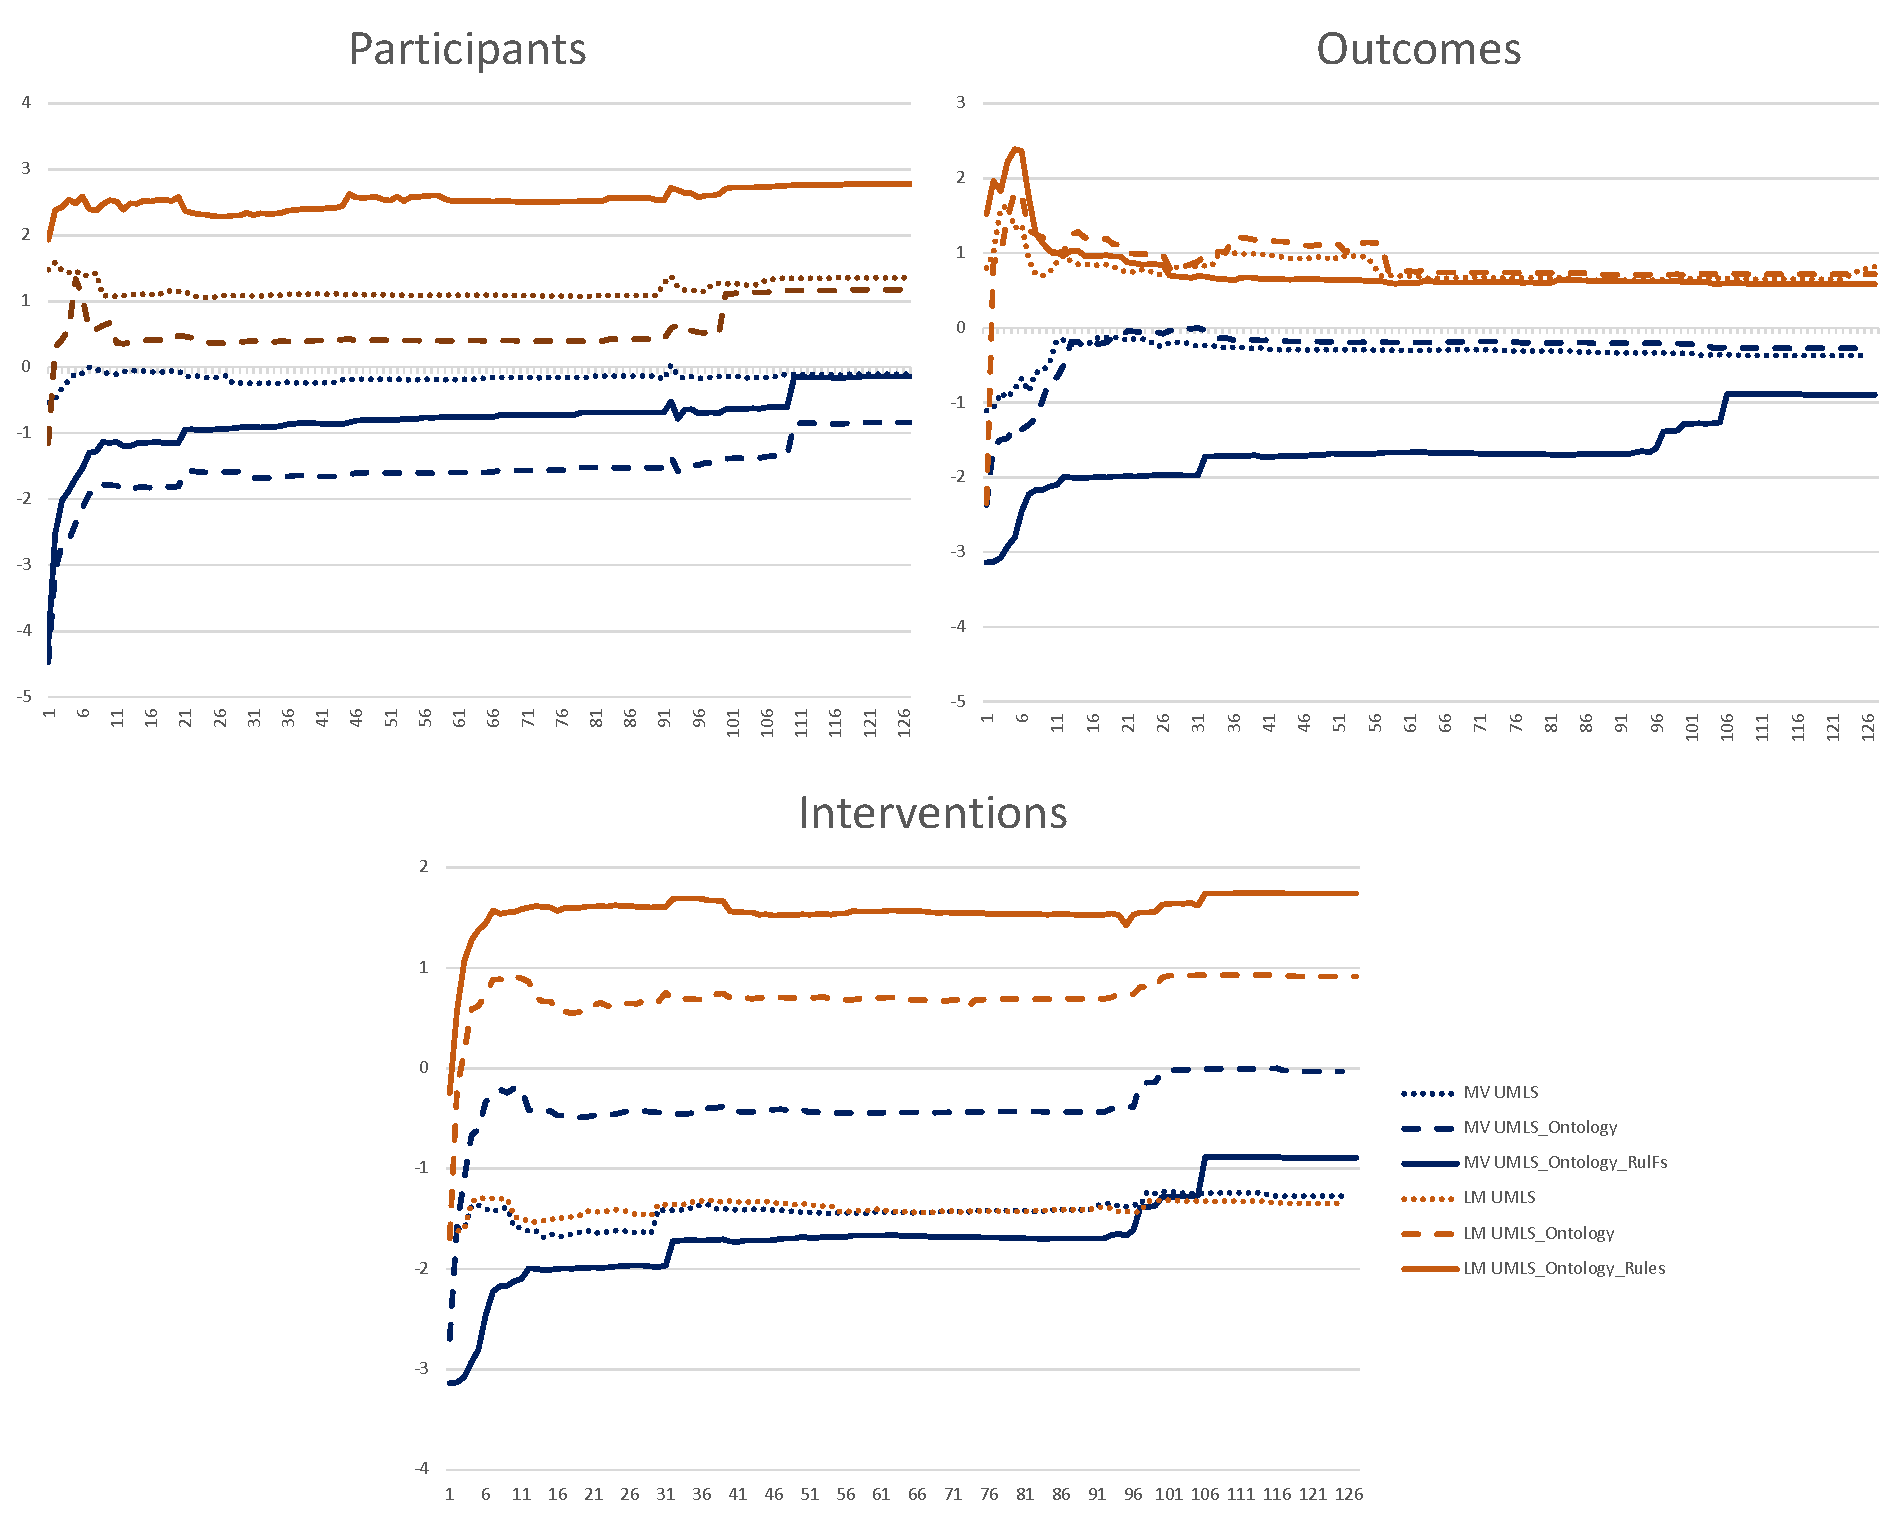
\includegraphics{figures/partitions.pdf}
    \caption{The relationship between the number of UMLS partitions and the macro-averaged F1 score for i) Participants target, ii) Interventions target and iii) Outcomes target.}
    \label{fig:partitions}
\end{figure}
%
%
%
%==============================
\section{DISCUSSION}\label{discussion}
%==============================
%
Our experiments show that weak-PICO approach to weakly supervised PICO extraction shows promising results for this challenging entity recognition task.
However, it is not straightforward to design labelling functions corresponding to the PICO targets, given their fuzzy nature and errors in the EBM-PICO gold test set.
It is easy to re-purpose the low-cost ontologies but challenging to map them to our fuzzy targets, which is shown by a decreased or stagnant F1 after adding non-UMLS ontologies.
Task-specific ReGeX and heuristics were developed upon inspection of the most frequent terms in the EBM-PICO validation set.
The same procedure was followed across the targets, but the performance boost using these LFs was only observed in the the participants and interventions and was detrimental to the outcomes.


Even though LM improves performance compared to MV, MV has a higher recall across experiments indicating a good corpus coverage of the labelling functions.
While some studies press on PICO extraction being a recall-oriented task, this is debated in practice.
In practice, high recall might lead to an accompanying high false positive (FP) rate, leading to the reviewers spending more time to manually weed out FP noise than reading and annotating the abstract with the entities.~\cite{liu2021sent2span}
LM only considers the information encoded into the weak sources to label phrases from the training text but does not consider the contextual information around the phrases.
Transformers consider the contextual information and should generalize beyond the label models in theory.
It is empirically confirmed by the performance boost that PubMedBERT brings on top of the label model for some instances, but the WS outcomes extraction results refute it.
%
%
%
%==============================
\subsection{error analysis and rectification}\label{err_ana}
%==============================
%
We expound on the error categories and provide examples here.
An error falls under \textit{repeated mention} if one instance of an entity is marked, but another identical instance of the same entity in the same context is not marked within the abstract. 
The reason could be the EBM-PICO guidelines flaw where the annotators of fine-grained entity annotation were confined to only annotate within the longer span-level annotation.
Hence any annotation error missed by the coarse-grained annotators was continued by the fine-grained annotators.

An error falls under \textit{remains unannotated} if a token should have been annotated as an entity but was not.
In the Intervention class, a large portion of this category was constituted by the generic mentions of controls (placebo, saline), which were not annotated.
In the Participant class, patient ethnicity and other information like smoking status and pregnancy information (marked in the coarse-grained span) were not marked in the fine-grained entity.
The reason could be that there was no fine-grained class to categorize this information. 
In the Outcome class, the annotators missed several important outcomes (along with their repeated mention).

\textit{Conjunction connector} errors are the conjunctions occurring between two semantically separate entities but are falsely marked as entities.
For example, ``Nausea and vomiting'' are two separate outcomes marked as one by annotating the conjunction between them.
When falsely marked as an entity, punctuation succeeding the entity, an article, or a preposition preceding the entity fall under the \textit{punctuation/article} errors.
Extraneous tokens marked along with the entity tokens fall under \textit{extra information} category.
For example, in the phrase ``This trial demonstrated short-term efficacy of smokeless tobacco in combination with'', the annotators had marked ``short-term efficacy of smokeless tobacco'' as an outcome entity, but only ``short-term efficacy'' is an outcome entity.
In contrast ``smokeless tobacco'' is an intervention entity. 
In the intervention class, the annotation guidelines mentioned not annotating any part of the text that did not mention the intervention name.
The annotators often marked extraneous information like intervention dosage, frequency, route of administration and information about the intervention administrator.


A generic reference is a co-reference of an entity mentioned using different or similar (but not identical) words. 
A generic reference of an entity (and its repeated mention) in the same abstract was several times left unmarked by the annotators constituting a \textit{generic reference} error.
For example, if the outcome endpoint ``smoking cessation'' was referred to in the same abstract elsewhere as ``quitting smoking'', it was not marked even though it is a reference to the outcome phrase ``smoking cessation''.
If ``aerobic exercise'' mentioned as ``exercise intervention'' was not marked, this also constitutes a generic reference error.
For instance, in an RCT, if ``breast cancer risk counselling'' intervention was referred to as ``risk counselling'', the former was marked, and the latter was missed.
This error was pronounced specially for the non-pharmaceutical interventions and outcomes.

An \textit{inconsistency} error arises when an entity is fully marked in some abstracts vs in the other abstracts the same entity is partially marked. 
For example, if an exercise intervention involved aerobic exercise involving stretching and running, this information (``stretching'', ``running'') was marked in some studies while not in the other studies.
In the case of the Participant class, the sample size sub-grouping information was inconsistently marked.
In another example, participant sample size information was either partially or completely marked (``59'' vs ``59 subjects'', ``200'' vs ``200 controls'').
In the Outcome class, the annotation guidelines marked ``what was measured and how it was measured''. 
Several times, the method used for measuring outcomes was inconsistently marked.
A \textit{junk} error is a token entirely irrelevant to an entity but is marked as one.
For example, in the Outcomes evaluation, the phrase ``evaluate and compare'' from the larger phrase ``This study aimed to evaluate and compare'' was marked as an outcome entity even though it is not a valid outcome.


These errors and inconsistencies in the EBM-PICO gold test (and training) set can cause faulty evaluation of the machine learning approaches defying the purpose of the corpus.
A possible reason behind these inconsistencies in the EBM-PICO corpus could be that the annotators had clinical background but lacked an informatics background.
This situation could undermine the importance of semantic consistency required for annotating such corpora.
Hiring annotators with the combined knowledge of clinical and informatics domains might improve the manual annotation quality.
The errors for PIO categories were rectified, and the updated dataset will be made available on Zenodo.
%
%
%
%==============================
\section{CONCLUSION}\label{conclusion}
%==============================
%
We adapted weak supervision for PICO spans and developed models for predicting PICO entities without a hand-labelled corpus.
We also identified errors pertinent to the current PICO benchmark, rectified them and used both datasets to evaluate the recognition models.
The approach achieves promising performance compared to full supervision and warrants further research into weak supervision for composite entities like PICO.
We firmly believe the approach could be extended to more clinical SR entities in the absence of a manually labelled corpus, thereby being a starting point to overcome the annotation bottleneck for SR entities.
In future, we will work on extending the data programming approach to the SR entities that do not have a manually labelled corpus like EBM-PICO and inspect strategies for mapping ontologies to PICO subclasses.
%
%
%
%==============================
\section{ACKNOWLEDGEMENTS}\label{acknowledgements}
%==============================
%
The authors thank Dr Jason A. Fries for his valuable comments and insights on the labelling function design and label model execution phase of the study. 
%
%
%
%==============================
\section{CONFLICT OF INTEREST STATEMENT}\label{conflictinterest}
%==============================
%
The authors have no conflicts of interest to declare.
%
%
%
%==============================
\section{FUNDING}\label{funding}
%==============================
%
The work was funded by HES-SO Valais-Wallis, Sierre, Switzerland.
%
%
%
%==============================
\section{ETHICS STATEMENT}\label{ethic}
%==============================
%
Our study focuses on the applicability of weak supervision for information extraction using publicly-available datasets.
Our investigation neither introduces any social or ethical concerns.
We do not foresee any direct social consequences or ethical issues.
%
%
%
%Where the bibliography will be printed
%==============================
\printbibliography
%
%\bibliography{literature}


%==============================
%
%
%
\end{document}